\section{Benefits of Tiny Tasks}
\label{sec:benefits}
\eat{Tiny tasks benefit data center workloads by providing inherent elasticity:
fine-grained units of work can be dynamically allocated to machines as
resources become available, eliminating stragglers and issues of data skew,
and allowing jobs to use available resources without sacrificing fairness
when new jobs are submitted.}

Tiny tasks benefit datacenter workloads by increasing the amount of elasticity
available to the scheduler: tiny tasks occupy resources for a very small
duration, so resources are allocated at a very fine granularity. This
allows resources to be dynamically reallocated between jobs, allowing greater
cluster utilization without sacrificing request latency, and to be dynamically
reallocated between tasks within a job, eliminating problems caused
by straggling tasks and data skew.

\subsection{Handling of skew and stragglers}
Prior studies~\cite{ananthanarayanan2010reining,zaharia2008improving} have noted that
task lengths in data parallel workloads are highly variable and that outlier
tasks negatively impact job completion time.
Outliers occur for one of two reasons.
First, outliers may be caused by poorly performing resources that cause the
task to take longer than if it had been run on a different machine; e.g.,
malfunctioning disks, contended CPUs, swapping memory, or congested networks.
Second, work may have been unevenly
divided across tasks, either due to
partitioning skew, where data was unevenly allocated to tasks, or due to
computational skew, where some data is more expensive to process.

Tiny tasks transform both the slow resources and the data skew problem
into a scheduling problem.  Rather than needing to predict which resources
are slow or statically partition data across tasks, a job is divided into
thosuands or millions of sub-second tiny tasks, and each task is scheduled
as resources become available.  In this manner, work is automatically
distributed evenly over available resources, without requiring complex skew
mitigation techniques: if a machine runs a computationally expensive task, it
will simply be assigned fewer total tasks.  Similarly, slow resources will
automatically be assigned less work, wihtout needing to predict which
resources are slow or which part of the network is congested.

\eat{
Tiny tasks help mitigate the effect of outliers in two ways. First, splitting
total work across a larger set of tasks more evenly partitions records across tasks, reducing data skew;
secondly, individual tasks can be moved in response to slow machines, network congestions, or
other cluster conditions, and run on other, faster machines.
}

To quantify these benefits, we used a Facebook trace to determine how much
job response time would improve if work were perfectly partitioned across
machines. For each job, we divided the total runtime for all tasks in the
job by the average number of slots used, and compare this ``binpacked''
completion time to the job's original completion time.
Figure~\ref{fig:binpacked}
demonstrates that jobs with 100 or more tasks benefit substantially from
balancing work more evenly across tasks: at the median, large jobs see
a \fixme{2.1}x reduction in response time from evenly spreading load
across tasks, and
jobs at the 95th percentile see a \fixme{5x} reduction in response time.
This experiment provides a conservative upper bound for two reasons. First, jobs
may have been using fewer than their fair share of slots in the original trace,
simply because there were not enough tasks to occupy more slots; in this case,
tiny tasks will further improve performance by increasing parallelism. Second,
if a task is running on a slow machine, it will take less total time when
broken into tiny tasks, because some of the tiny tasks will be run on faster
machines.

\begin{figure}[!t]
\centering
\hspace{2ex}
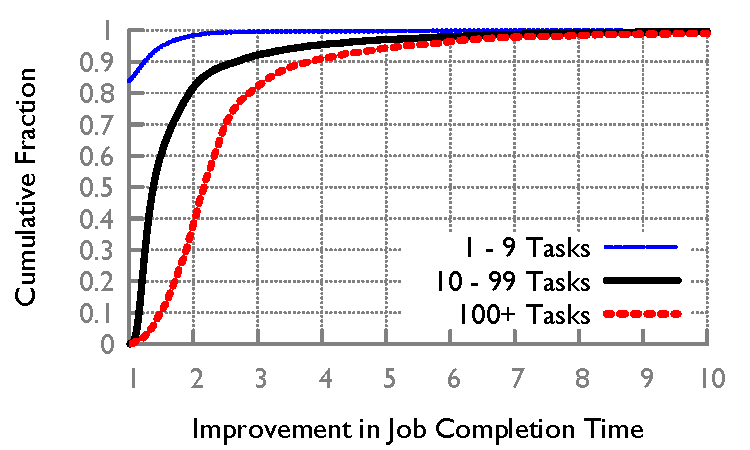
\includegraphics[width=0.5\textwidth]{figures/binpacked1-sep}
\vspace{-4ex}
\caption{Improvement from perfectly balancing the total machine time for the
job across tasks.}
\vspace{-2ex}
\label{fig:binpacked}
\end{figure}

\eat{Figure~\ref{fig:sparkskew} demonstrates the improvement offered by tiny tasks on a Spark MapReduce job with data skew and machines that exhibited a random 5x performance variance.
With tiny tasks, Spark is able to mitigate both skew and stragglers without explicit knowledge of machines' speeds or records' processing costs.}


\begin{figure}[!t]
\centering
\hspace{2ex}
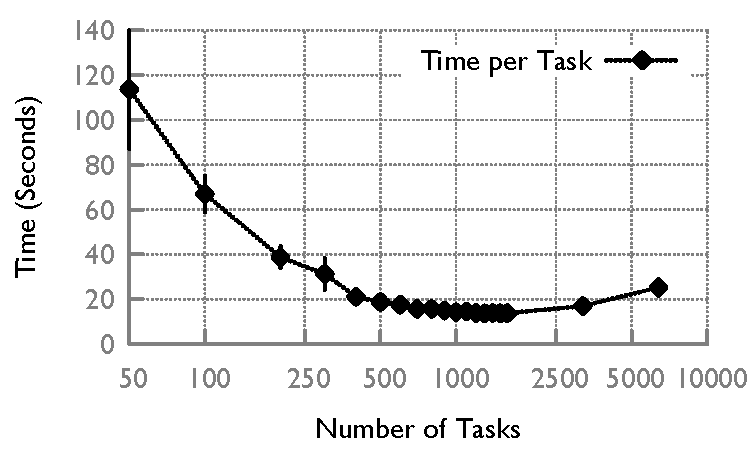
\includegraphics[width=0.5\textwidth]{figures/spark-skew-results}
\vspace{-4ex}
\caption{Improvement from using tiny tasks in a cluster where 20\% of machines
take 21x longer to run each task. Error bars depict standard deviation.}
\vspace{-2ex}
\label{fig:sparkskew}
\end{figure}



To demonstrate that using tiny tasks automatically avoids slow machines,
we modified some machines in a cluster to run more slowly, and then
ran a Spark job using different numbers of tasks. We used $50$ m1.medium EC2
instances, 10 of which were modified to take 21x longer to run each task.
Figure~\ref{fig:sparkskew} demonstrates that using a larger number of tasks
improves response time by \fixme{20x} compared to using the same number
of tasks as machines in the cluster, because the slow machines will be
assigned approximately $\frac{1}{21}$ as many tasks. At some point, due to
task launch overheads, using more tasks increases response time; we discuss
how to avoid this problem with a new cluster framework in \S\ref{sec:prog}.

\begin{figure*}[!t]
\centering
\subfigure[] {
    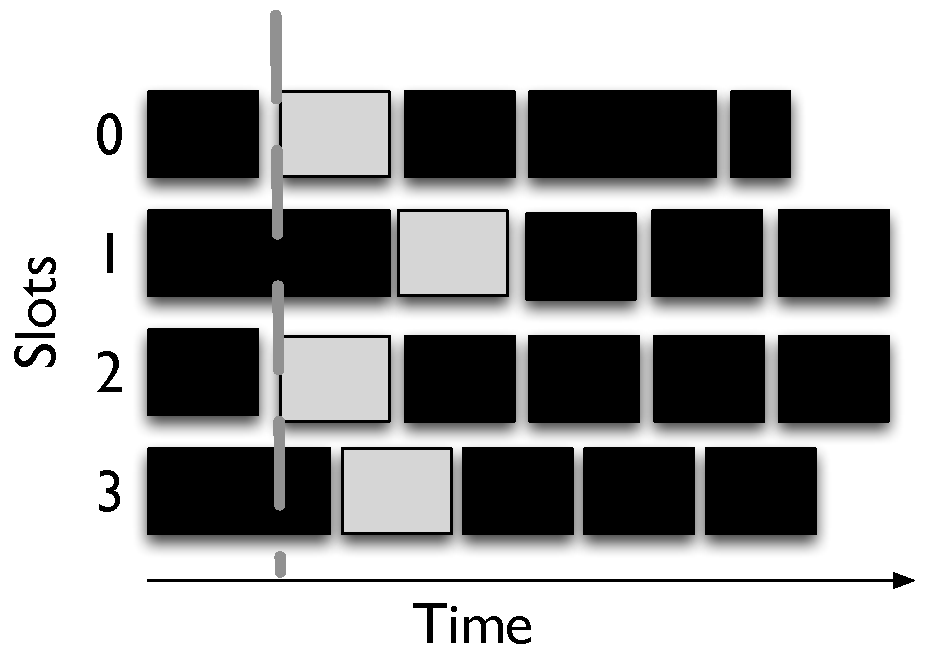
\includegraphics[width=0.4\textwidth]{figures/slot_diagram_before}
    \label{fig:slot_diagram_original}
}
\subfigure[] {
    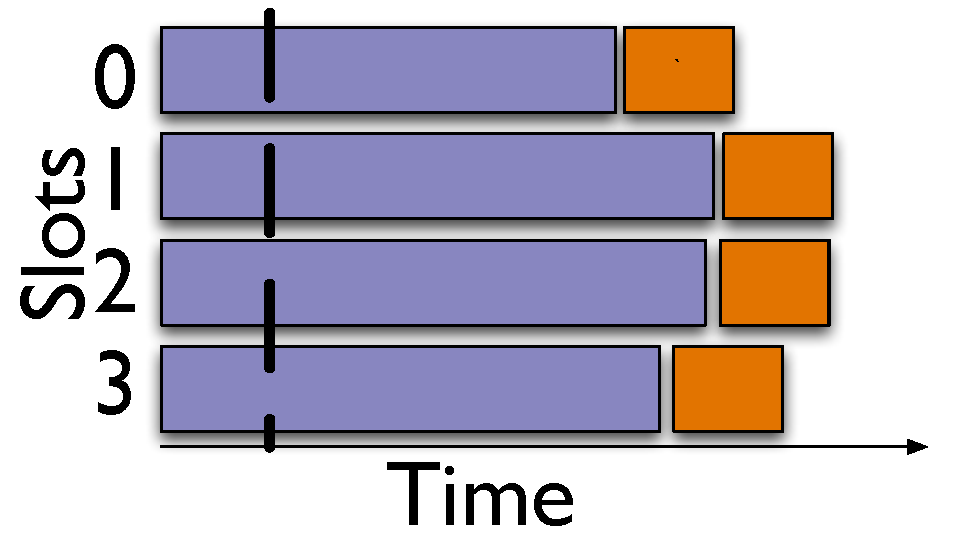
\includegraphics[width=0.4\textwidth]{figures/slot_diagram_after}
    \label{fig:slot_diagram_tiny}
}
\caption{Two jobs running in a cluster with four slots. With today's tasks,
tasks for the grey job need to wait for long-running tasks from the black job to
complete before they are launched, shown in (a).
On the other hand, with tiny tasks (shown in (b)), resource
allocation is fine-grained, so resources will quickly be allocated to new
jobs, allowing the grey job to complete more quickly.}
\vspace{-2ex}
\label{fig:slot_diagram}
\end{figure*}



\subsection{Response Time}
Today, sharing a cluster between interactive and batch jobs involves trading off
responsiveness and utilization. If a cluster is highly utilized,
an interactive job may need to wait for long-running batch tasks to
complete before it can be serviced; reserving slots for
interactive slots avoids this problem but results in lower utilization.
Using tiny tasks for all jobs avoids this tradeoff: the cluster can run at
high utilization, while
simultaneously guaranteeing that interactive jobs will only need to wait for
a short time before being serviced. Figure~\ref{fig:slot_diagram} depicts a simple example
with only two jobs, and demonstrates that with tiny tasks, a newly arriving
job can quickly gain its fair share of resources, even in the presence
of large, batch jobs.
